\appendix
\chapter{Prílohy}

\section{GUI}
{ \hspace*{-0.3in}
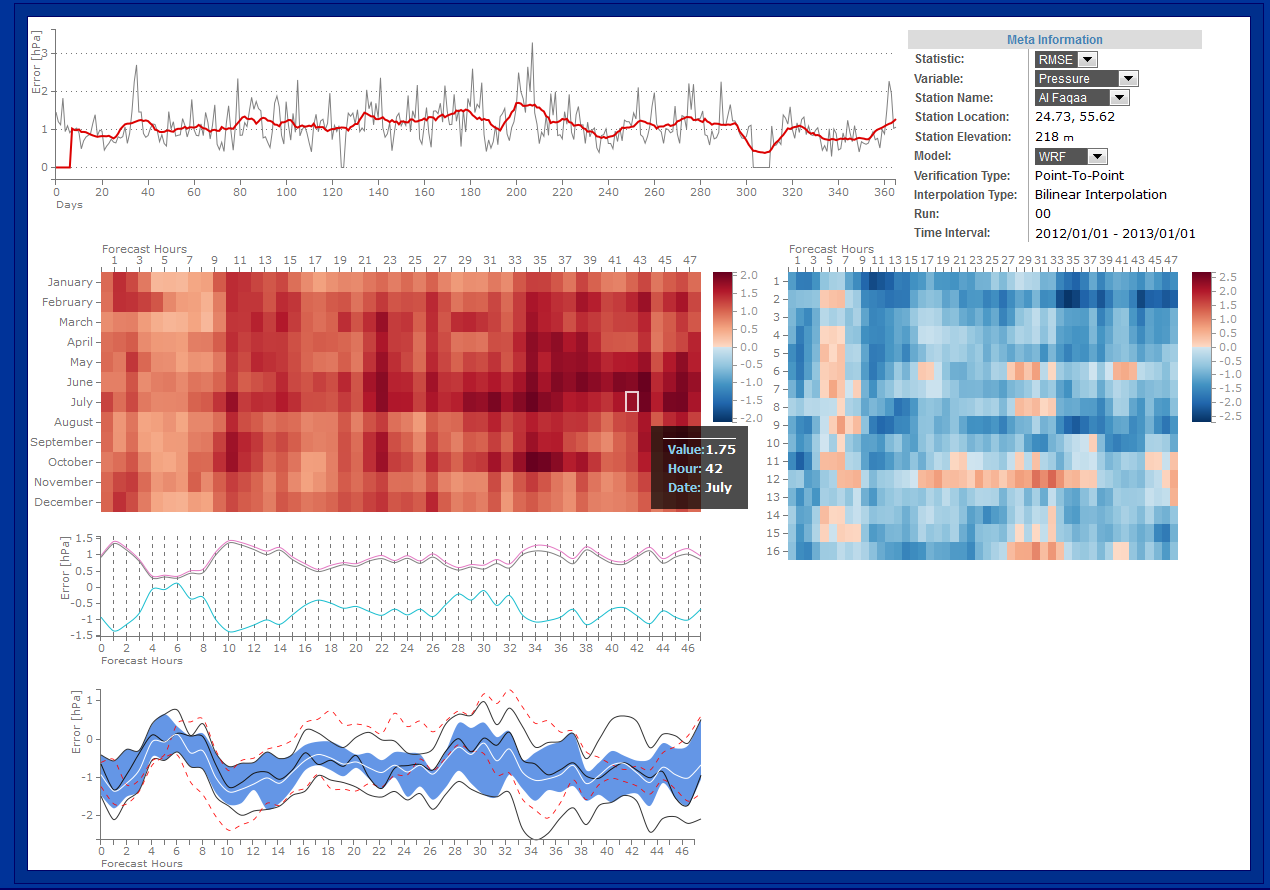
\includegraphics[width=7in]{gui} 
}
Grafické užívateľské rozhranie našej aplikácie pozostáva pozostáva z jednotlivých prvkov, tak ako sme to opísali v podsekcii \ref{subsec:flatlayout}. V pravom hornom rohu si v tabuľke meta informácií môže užívateľ zvoliť zobrazovanú štatistiku, veličinu, stanicu a predpovedný model, ktorý chce verifikovať. Kliknutím na konkrétny mesiac sa užívateľovi zobrazia grafy pre daný mesiac.

\section{Príklad vizualizácie starého systému}
\label{sec:oldsys}
{ 	\centering
	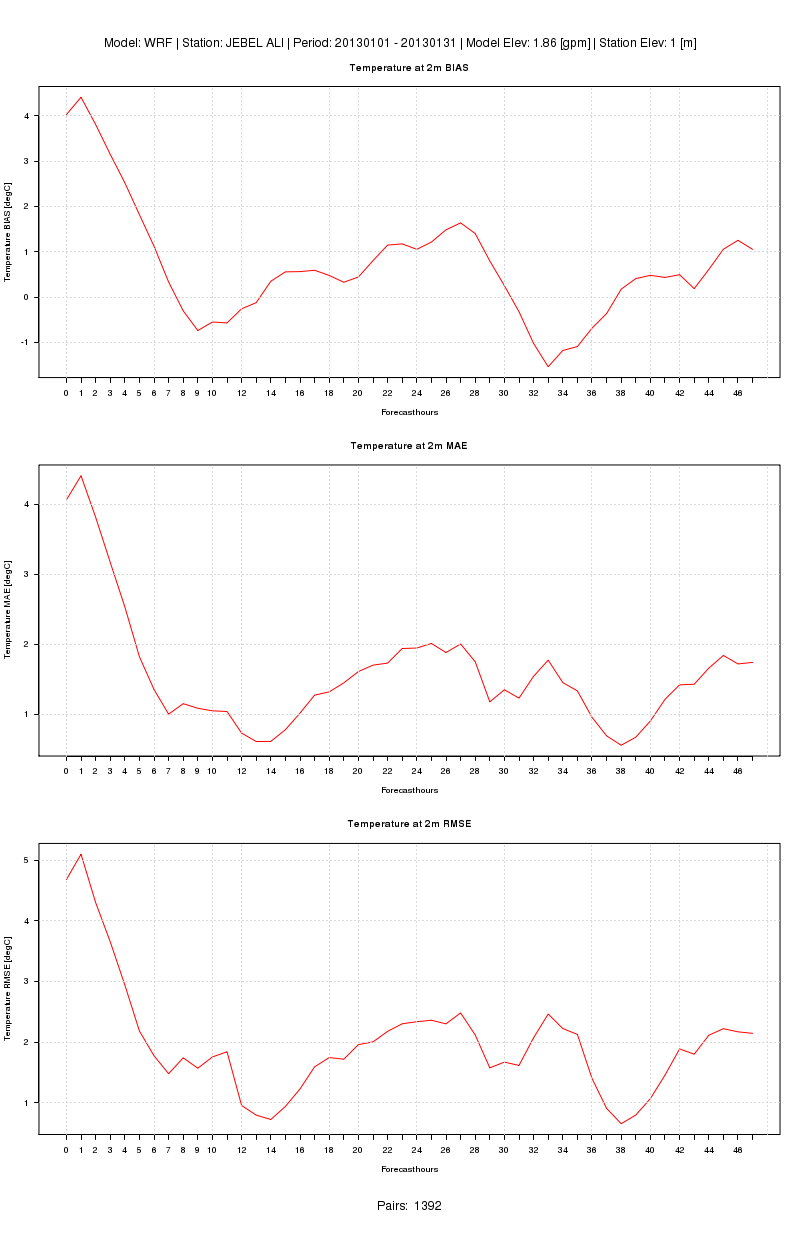
\includegraphics[width=3in]{oldsys} 
} \\
V predošlom systéme verifikovania sa jednotlivé štatistiky vizualizovali pomocou čiarových diagramov a to jeden diagram pre každú štatistiku. Jednotlivé grafy sa generovali pomocou skriptovacieho jazyka R (pozri \ref{subsec:R}) do statických obrázkov bez možnosti interakcie.

\section{Testovací formulár}
\label{sec:testform}
{
\hspace*{-1in}
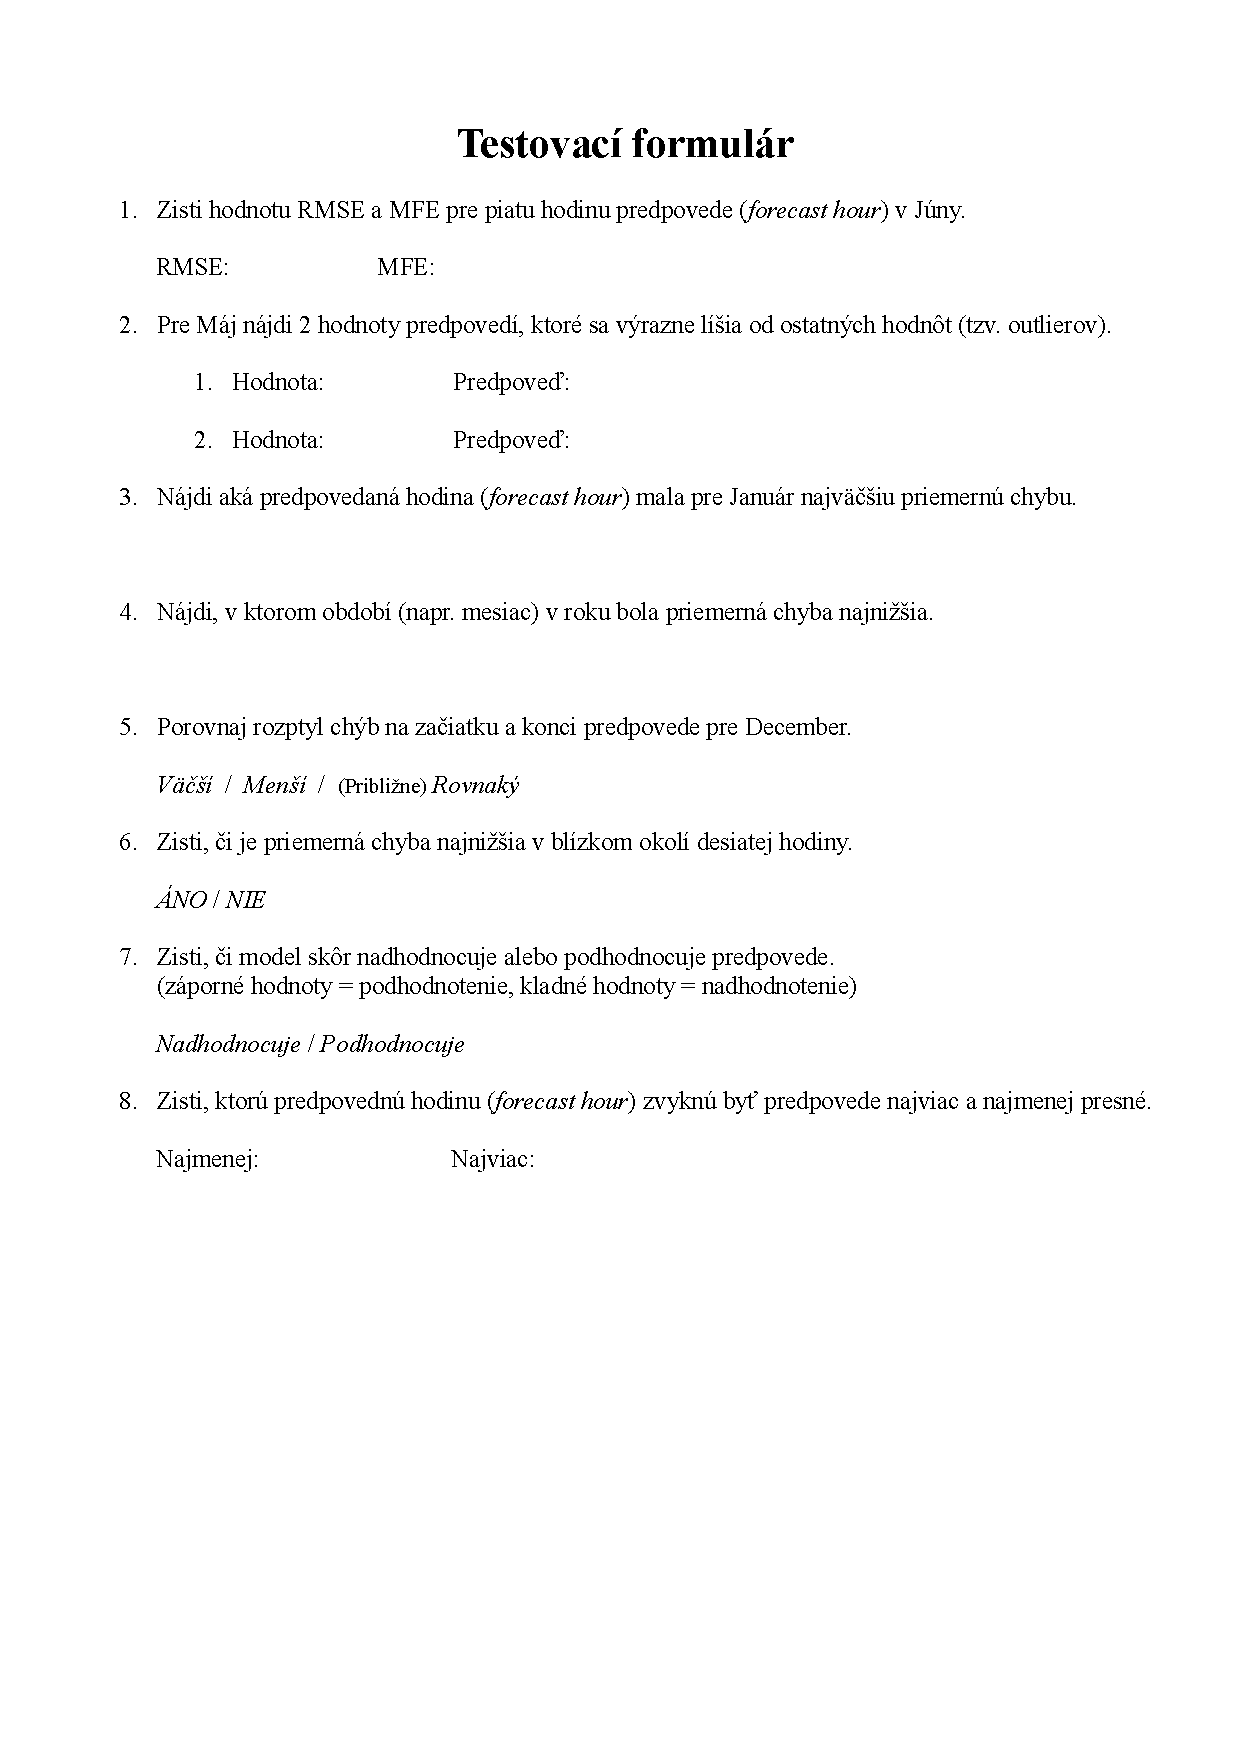
\includegraphics[width=597pt,height=780pt]{testform}
}
% 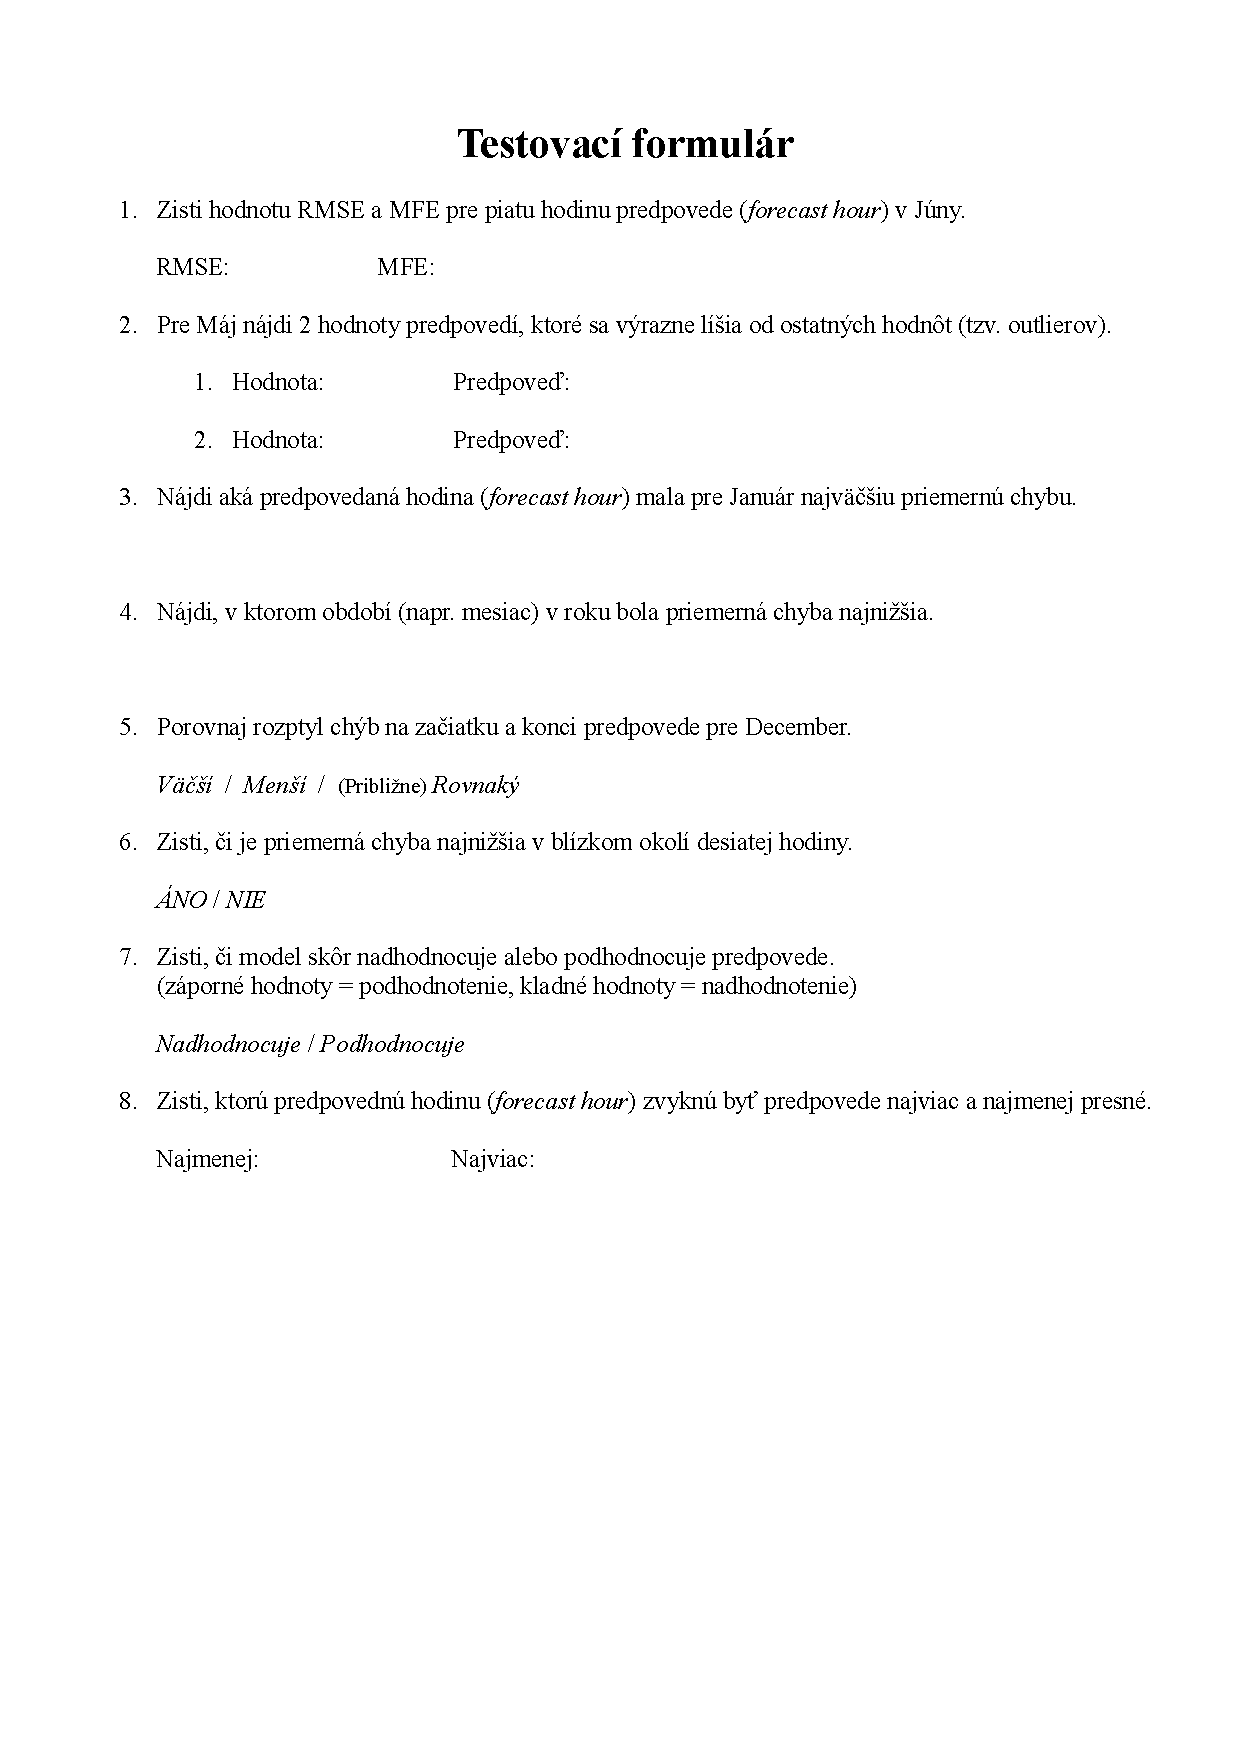
\includepdf[pages={1}]{testform.pdf}


\section{CD}
Obsah CD:
\begin{easylist}[itemize]
	# Zdrojové súbory
	# Testovacie dáta
	# Elektronická verzia práce
\end{easylist}